\section{Robustez Estatística e Ablação de Atributos}\label{sec:robustez_resultados}

As métricas anteriores descrevem o desempenho observado em um único período contínuo de 365 dias. Esta seção acrescenta três verificações: incerteza das métricas sob dependência temporal, contribuição incremental dos grupos de atributos e estrutura remanescente nos resíduos. Todas reutilizam as previsões e o corte oficial de $h=1$; nenhuma observação do teste é incorporada ao treinamento dos modelos originais.

\subsection{Intervalos de Confiança das Métricas}\label{sec:resultados_bootstrap}

A Tabela~\ref{tab:intervalos_bootstrap} apresenta intervalos percentis de 95\% obtidos com 10.000 réplicas de \textit{block bootstrap} circular e blocos de sete dias. Os intervalos são largos porque o erro diário é heterogêneo e parte relevante do MAE se concentra em poucos períodos chuvosos e dias de alto volume. Eles quantificam a incerteza da métrica no recorte observado, não a faixa de uma previsão individual.

\begin{table}[H]
\centering
\caption{Métricas e intervalos de 95\% por \textit{block bootstrap} semanal}
\label{tab:intervalos_bootstrap}
\small
\begin{tabular}{lrrrr}
\toprule
\textbf{Modelo} & \textbf{MAE} & \textbf{IC95\% do MAE} & \textbf{RMSE} & \textbf{IC95\% do RMSE} \\
\midrule
XGBoost & 61,47 & [49,97; 74,64] & 99,73 & [74,89; 124,68] \\
Bi-LSTM & 61,74 & [51,69; 73,42] & 99,83 & [75,88; 124,58] \\
Bi-GRU & 62,10 & [52,10; 73,66] & 96,90 & [75,05; 119,60] \\
Persistência & 68,59 & [56,80; 82,48] & 105,61 & [80,41; 131,54] \\
\bottomrule
\end{tabular}
\par\smallskip
{\small Fonte: Elaborado pelos autores (2026). Blocos de sete dias, 10.000 réplicas e semente 42.\par}
\end{table}

\begin{figure}[H]
    \centering
    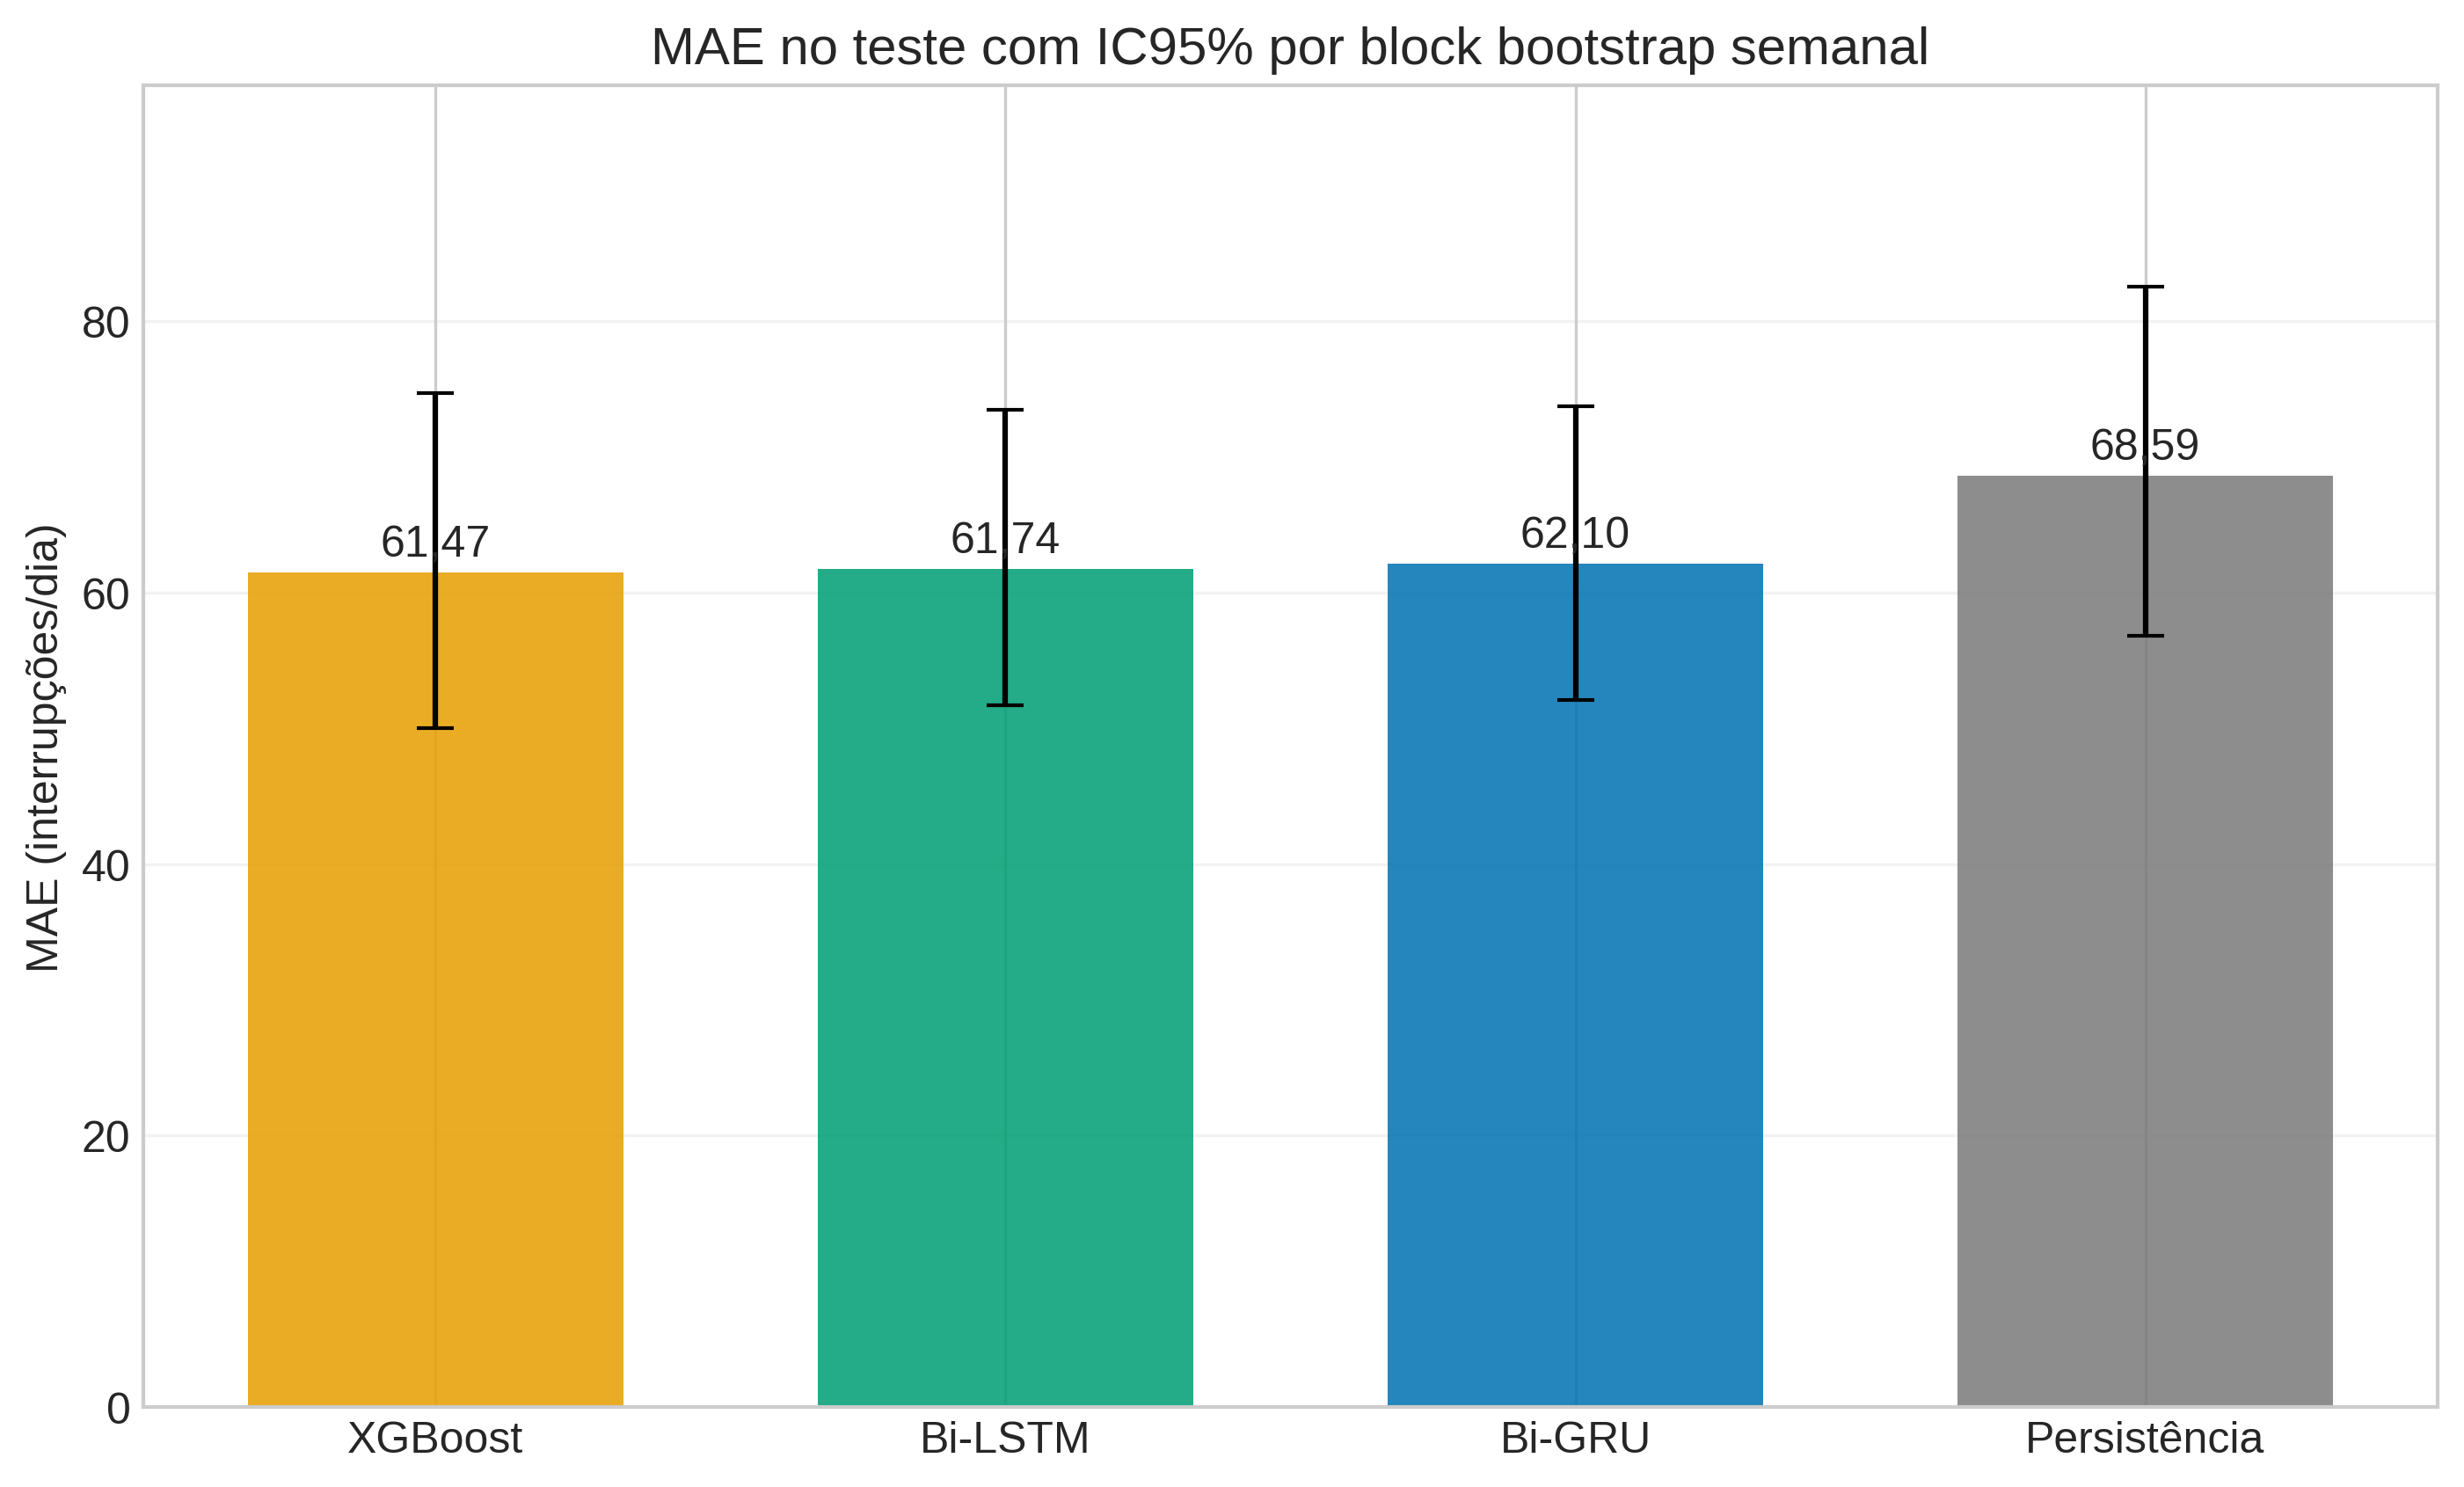
\includegraphics[width=0.92\textwidth]{img/uncertainty_mae_block_bootstrap.png}
    \caption{MAE observado e intervalos percentis de 95\% sob \textit{block bootstrap} semanal.}
    \small{Fonte: Elaborado pelos autores (2026).}
    \label{fig:incerteza_mae_bootstrap}
\end{figure}

A proximidade entre os três modelos treinados fica mais clara quando a comparação é pareada. Na Tabela~\ref{tab:contrastes_modelos}, $\Delta\mathrm{MAE}_{A-B}<0$ favorece o modelo $A$. Os contrastes XGBoost--Bi-LSTM, XGBoost--Bi-GRU e Bi-LSTM--Bi-GRU estão próximos de zero, e seus intervalos contêm zero. Portanto, embora cada arquitetura lidere uma ou mais métricas pontuais, o teste não separa seus MAEs no período avaliado.

\begin{table}[H]
\centering
\caption{Contrastes pareados de MAE entre modelos no teste principal}
\label{tab:contrastes_modelos}
\small
\begin{tabular}{llrr}
\toprule
\textbf{Alternativa A} & \textbf{Alternativa B} & $\boldsymbol{\Delta}$\textbf{MAE A--B} & \textbf{IC95\%} \\
\midrule
XGBoost & Bi-LSTM & $-0,26$ & [$-8,11$; 7,82] \\
XGBoost & Bi-GRU & $-0,63$ & [$-8,75$; 7,81] \\
Bi-LSTM & Bi-GRU & $-0,37$ & [$-4,96$; 4,14] \\
XGBoost & Persistência & $-7,11$ & [$-15,03$; 1,37] \\
Bi-LSTM & Persistência & $-6,85$ & [$-14,53$; 0,67] \\
Bi-GRU & Persistência & $-6,48$ & [$-14,02$; 1,20] \\
\bottomrule
\end{tabular}
\par\smallskip
{\small Fonte: Elaborado pelos autores (2026). Valor negativo favorece A.\par}
\end{table}

Os três modelos apresentam ganhos pontuais de aproximadamente 6,5 a 7,1 interrupções por dia sobre a persistência, mas os intervalos semanais desses contrastes também contêm zero. Ao ampliar o bloco para 14 e 30 dias, as comparações entre XGBoost, Bi-LSTM e Bi-GRU continuam contendo zero. Alguns contrastes contra a persistência mudam de classificação conforme o comprimento adotado. Essa sensibilidade impede transformar a vantagem pontual observada sobre a referência em uma afirmação inferencial geral, embora todos os valores centrais permaneçam favoráveis aos modelos treinados.

O resultado altera a leitura da Tabela~\ref{tab:metricas_modelos}: não existe evidência, neste teste, para ordenar os três modelos pelo MAE com segurança estatística. As diferenças de RMSE, $R^2$ e MAPE continuam úteis para caracterizar o tipo de erro, mas não eliminam a incerteza associada ao período e à dependência temporal.

\subsection{Ablação dos Grupos de Atributos no XGBoost}\label{sec:resultados_ablacao}

A ablação examina uma pergunta distinta da importância por ganho: quanto cada grupo acrescenta ao desempenho fora da amostra quando o algoritmo, os hiperparâmetros e o corte temporal são mantidos. A Tabela~\ref{tab:ablacao_xgboost} apresenta os resultados das cinco variantes do XGBoost e da persistência.

\begin{table}[H]
\centering
\caption{Ablação dos grupos de atributos no XGBoost para $h=1$}
\label{tab:ablacao_xgboost}
\small
\begin{tabular}{lrrrrr}
\toprule
\textbf{Variante} & \textbf{Atributos} & \textbf{MAE} & \textbf{RMSE} & $\boldsymbol{R^2}$ & \textbf{MAPE (\%)} \\
\midrule
Completo & 41 & 61,47 & 99,73 & 0,409 & 20,38 \\
Histórico + calendário & 10 & \textbf{54,26} & \textbf{97,18} & \textbf{0,439} & \textbf{16,69} \\
Clima + calendário & 36 & 79,22 & 124,70 & 0,076 & 24,89 \\
Somente histórico & 5 & 61,17 & 100,44 & 0,400 & 19,65 \\
Somente calendário & 5 & 75,32 & 126,38 & 0,051 & 21,11 \\
Persistência & 1 & 68,59 & 105,61 & 0,337 & 22,37 \\
\bottomrule
\end{tabular}
\par\smallskip
{\small Fonte: Elaborado pelos autores (2026). As cinco variantes do XGBoost reutilizam os hiperparâmetros do modelo completo.\par}
\end{table}

\begin{figure}[H]
    \centering
    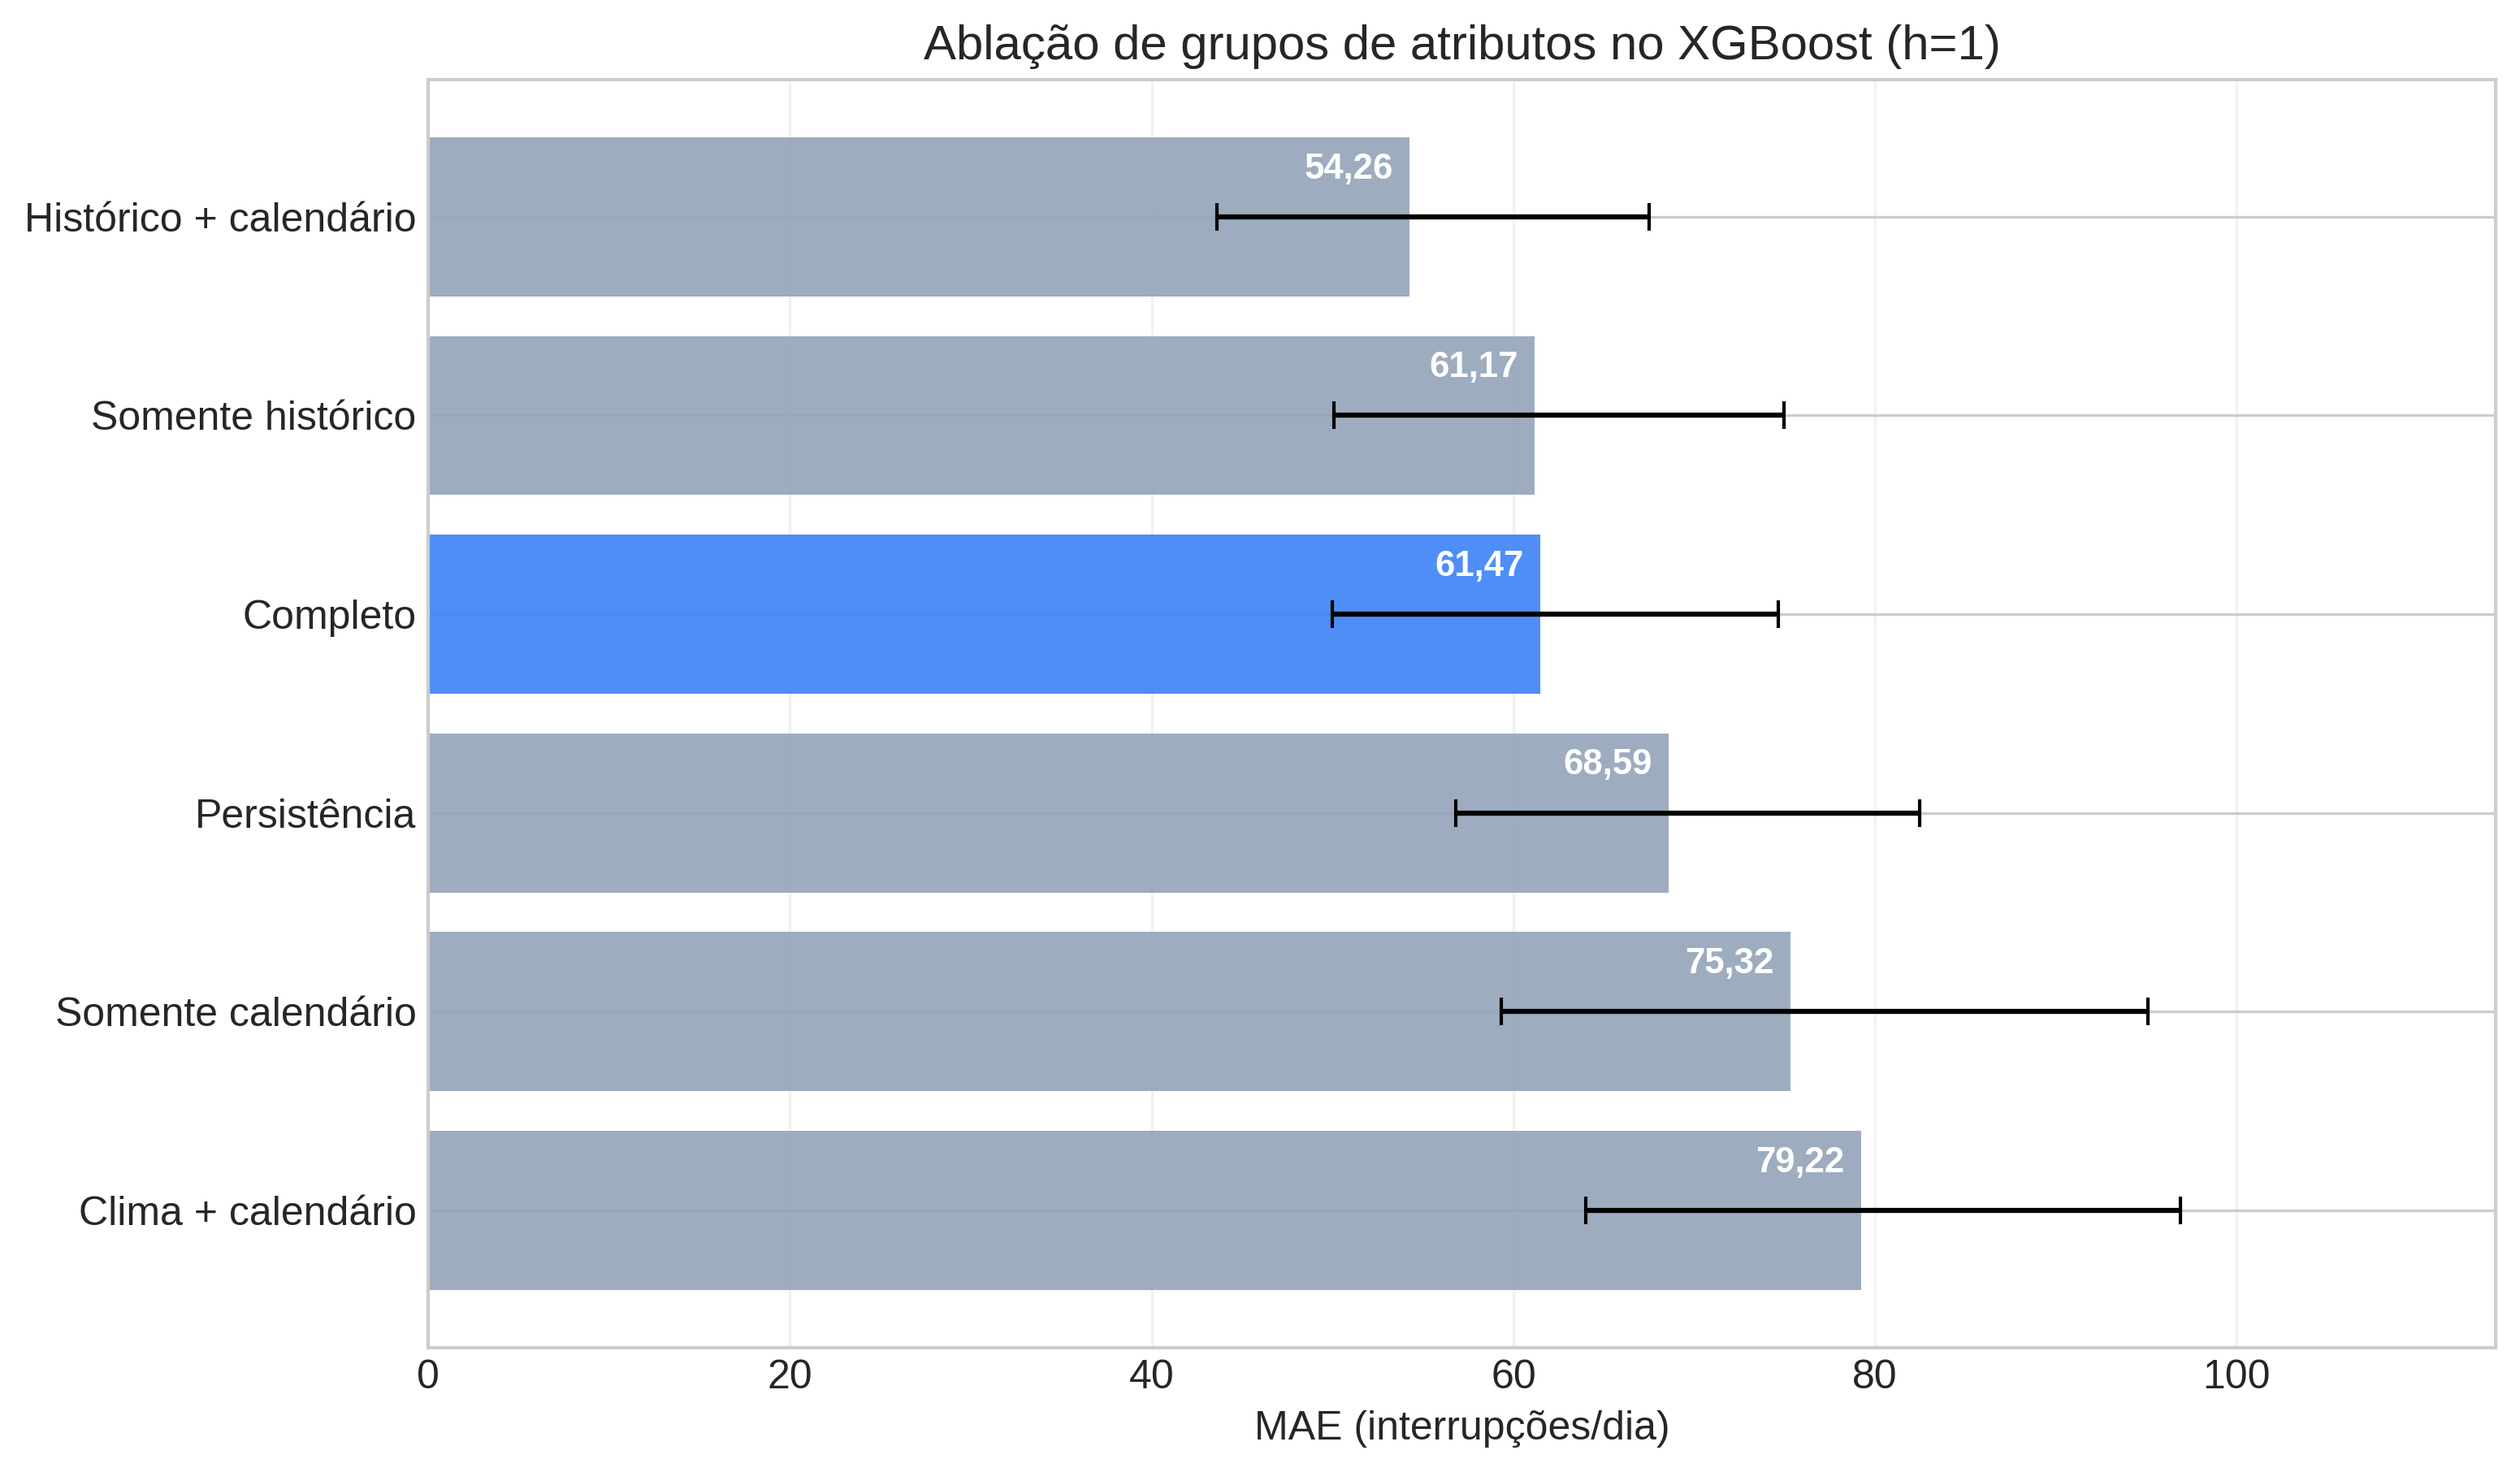
\includegraphics[width=0.94\textwidth]{img/ablation_xgboost.png}
    \caption{MAE e IC95\% das variantes de ablação do XGBoost e da persistência.}
    \small{Fonte: Elaborado pelos autores (2026).}
    \label{fig:ablacao_xgboost}
\end{figure}

O menor erro foi obtido por \textbf{histórico + calendário}: MAE 54,26, RMSE 97,18, $R^2=0{,}439$ e MAPE 16,69\%. Em comparação com o modelo completo, a redução pontual do MAE foi de 7,21 interrupções por dia. Sob blocos de sete dias, o intervalo pareado foi [$-14,82$; $-0,83$]; com 14 dias, [$-16,90$; $-0,33$]. Com blocos de 30 dias, o limite superior alcançou 0,11 e o intervalo passou a conter zero, indicando que a força inferencial do contraste depende da escala de dependência preservada.

A variante de \textbf{somente histórico} apresentou MAE 61,17, praticamente igual ao completo (diferença $-0,30$; IC95\% [$-8,39$; 6,70]). Acrescentar o calendário ao histórico reduziu o MAE em 6,91, com IC95\% [$-9,72$; $-4,23$] no esquema semanal. Esse padrão indica que o ciclo anual e a posição no calendário complementam o nível recente da série no recorte avaliado.

Em sentido oposto, \textbf{clima + calendário}, sem o histórico do alvo, obteve MAE 79,22, superior ao modelo completo e à persistência. A diferença contra o completo foi 17,74, com IC95\% [10,75; 25,34] sob blocos de sete dias e permaneceu acima de zero nas sensibilidades de 14 e 30 dias. Contudo, clima + calendário não foi claramente distinto de somente calendário: a inclusão das 31 variáveis meteorológicas alterou o MAE em 3,90, com IC95\% [$-8,01$; 17,56].

Esses resultados mostram que o \textbf{histórico das interrupções é o principal portador de informação preditiva em $h=1$}. As variáveis climáticas apresentam associações exploratórias e algumas aparecem no ranking de ganho do modelo completo, mas o grupo climático não forneceu ganho incremental no teste de ablação. Isso não demonstra irrelevância física do clima. A estação única, a agregação distrital diária, a ausência de previsão meteorológica espacial e a correlação entre atributos podem impedir que o sinal físico se converta em melhoria preditiva adicional.

A variante de menor MAE não substitui o modelo oficial. Ela foi identificada numa análise pós-hoc sobre o mesmo teste, e promovê-la retroativamente configuraria seleção orientada pelo conjunto de avaliação. O resultado gera uma hipótese verificável para um período futuro: um XGBoost mais parcimonioso, baseado em histórico e calendário, deve ser comparado prospectivamente ao modelo completo e a uma especificação meteorológica espacialmente mais rica.

\subsection{Dependência Temporal Remanescente nos Resíduos}\label{sec:resultados_residuos_temporais}

A Tabela~\ref{tab:diagnostico_residual_temporal} complementa a KDE e a heteroscedasticidade com viés e autocorrelação. Como o resíduo foi definido por $e_t=y_t-\widehat y_t$, valores médios positivos indicam subestimação. Os intervalos de viés dos quatro modelos contêm zero: XGBoost [$-13,83$; 14,50], Bi-LSTM [$-7,86$; 20,54], Bi-GRU [$-20,97$; 7,04] e persistência [$-5,33$; 5,62]. Assim, não se identifica viés médio global claramente diferente de zero.

\begin{table}[H]
\centering
\caption{Viés e dependência temporal dos resíduos no teste principal}
\label{tab:diagnostico_residual_temporal}
\small
\begin{tabular}{lrrrrrr}
\toprule
\textbf{Modelo} & \textbf{Viés médio} & \textbf{Mediana} & \textbf{DP} & $\boldsymbol{\rho_1}$ & $\boldsymbol{\rho_7}$ & $\boldsymbol{p_{LB}(14)}$ \\
\midrule
XGBoost & 0,26 & $-4,92$ & 99,86 & 0,238 & 0,140 & $9,04\times10^{-9}$ \\
Bi-LSTM & 5,36 & $-3,62$ & 99,82 & 0,304 & 0,110 & $3,96\times10^{-9}$ \\
Bi-GRU & $-7,94$ & $-19,32$ & 96,70 & 0,362 & 0,022 & $2,17\times10^{-9}$ \\
Persistência & $-0,03$ & $-1,00$ & 105,75 & $-0,223$ & 0,139 & $1,35\times10^{-7}$ \\
\bottomrule
\end{tabular}
\par\smallskip
{\small Fonte: Elaborado pelos autores (2026). $p_{LB}(14)$: valor-$p$ do teste de Ljung--Box até 14 dias.\par}
\end{table}

\begin{figure}[H]
    \centering
    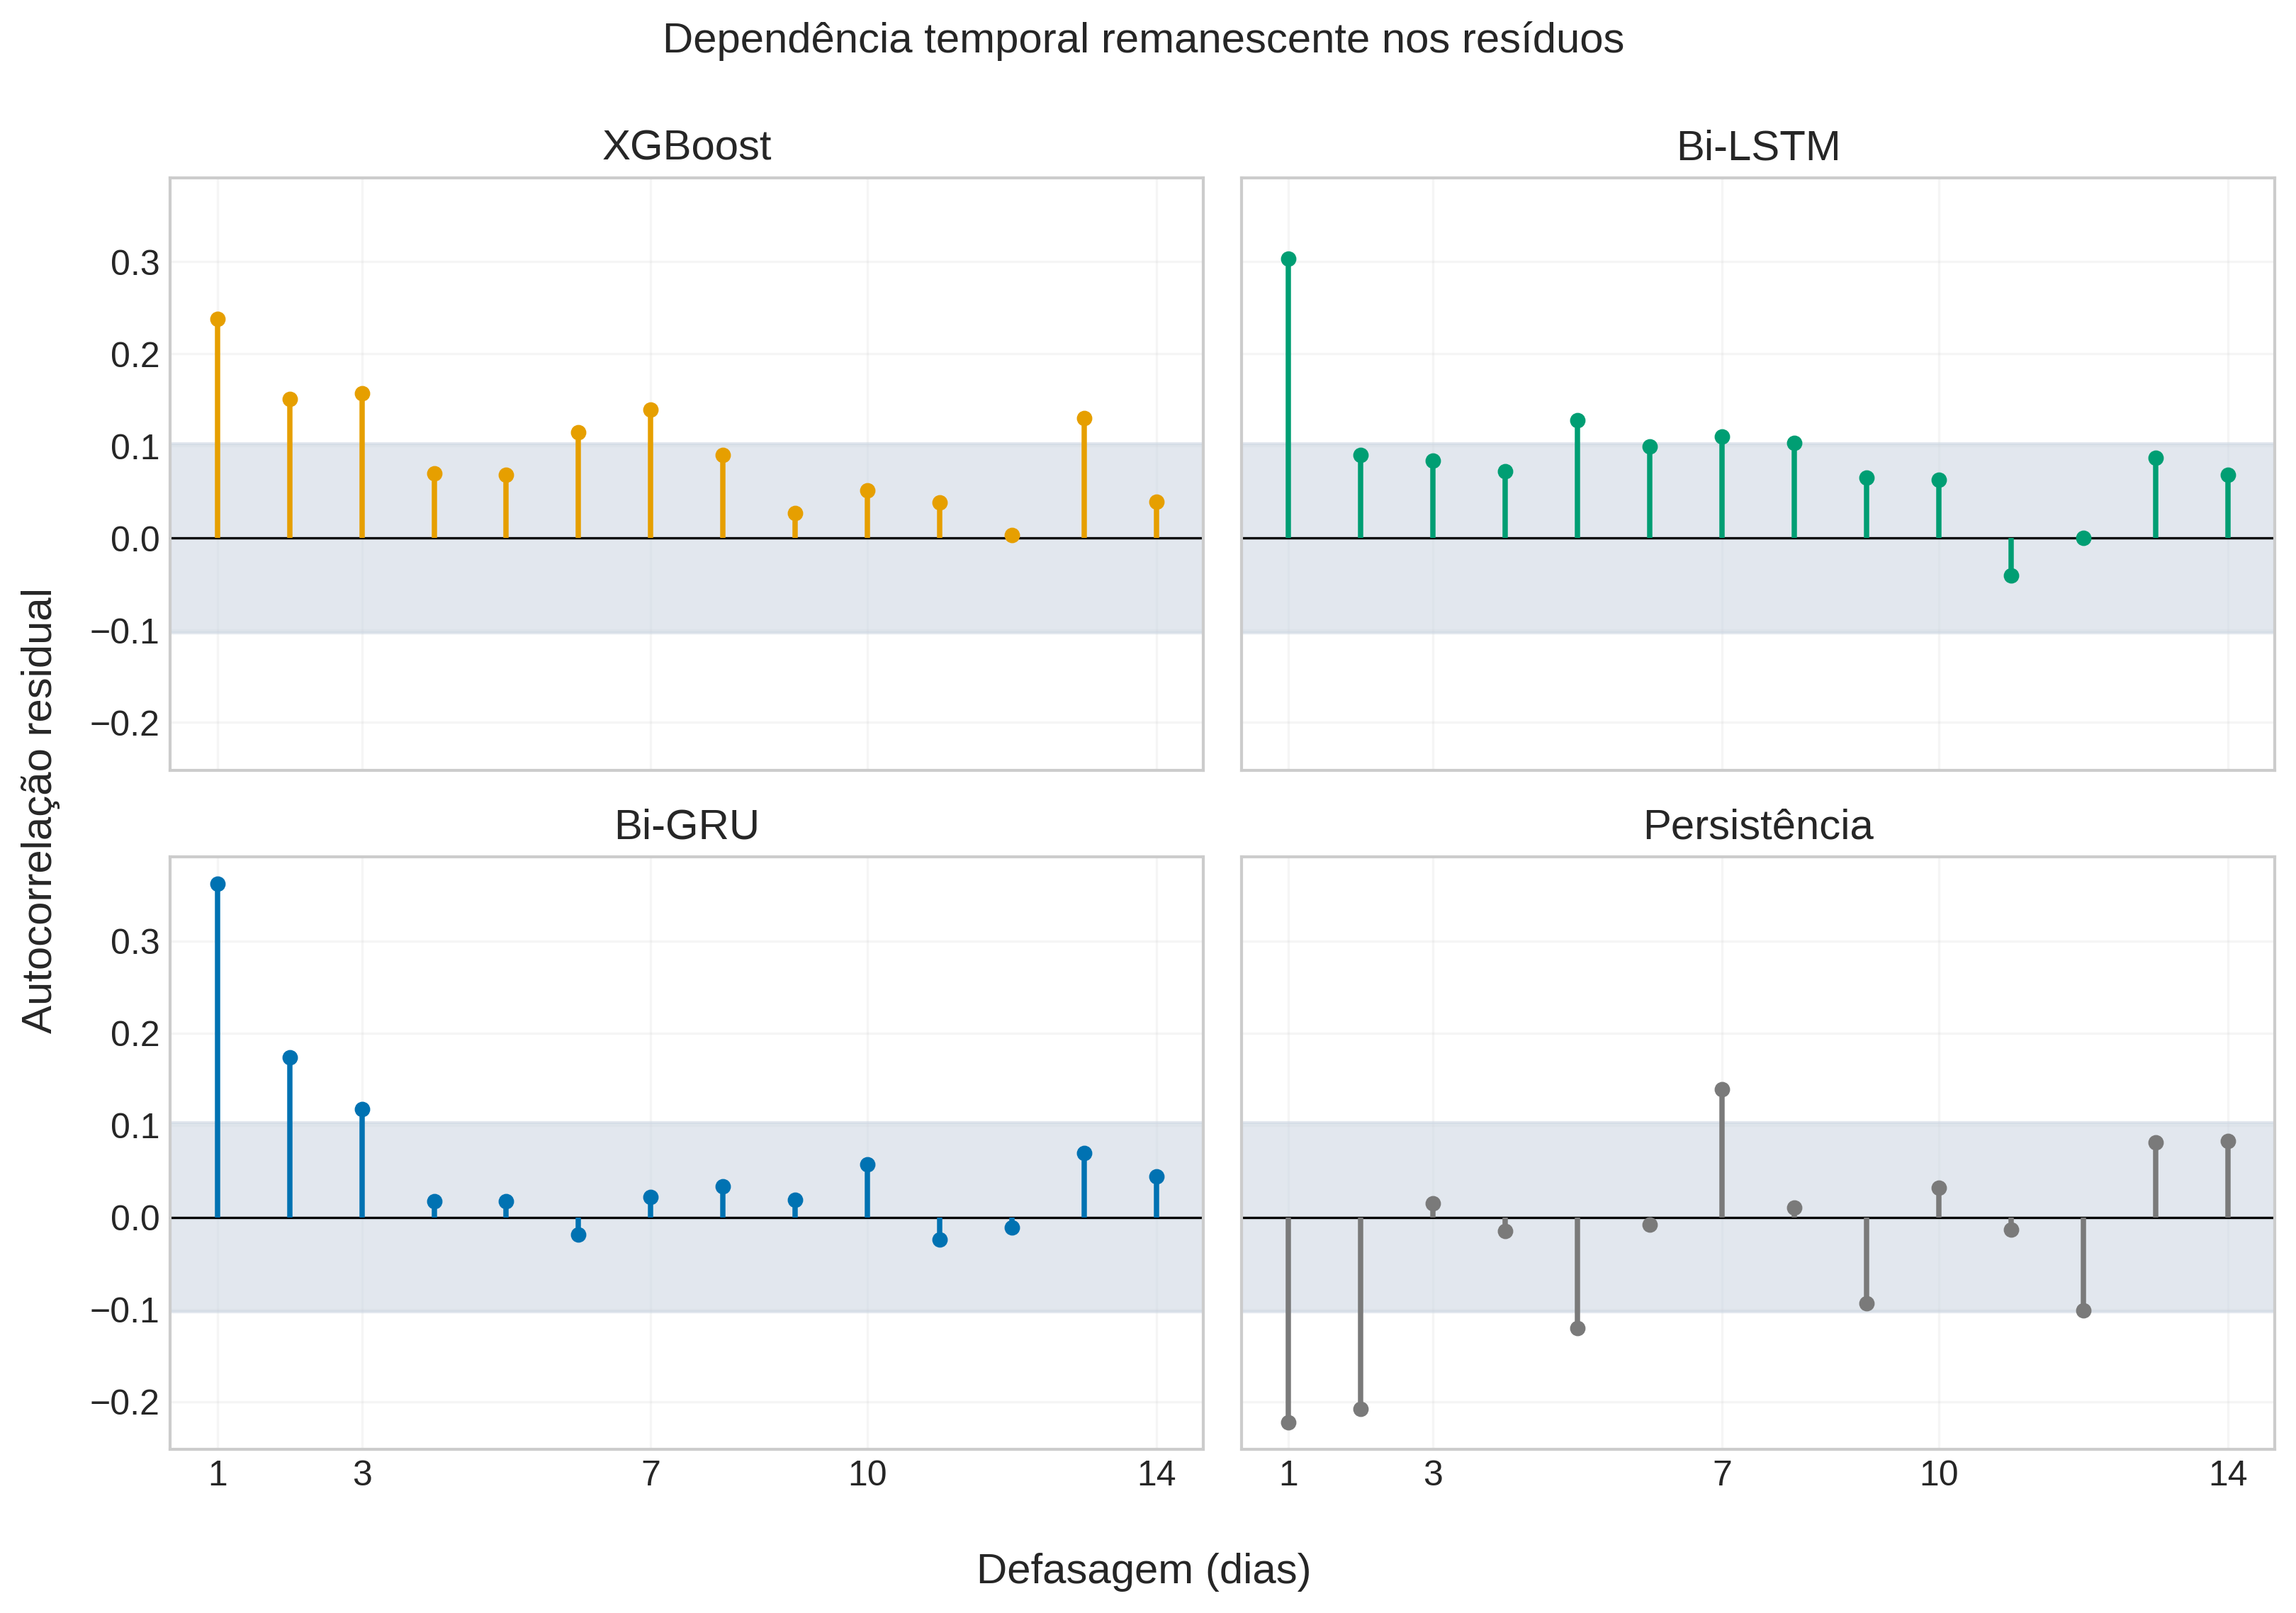
\includegraphics[width=0.96\textwidth]{img/residual_acf_models.png}
    \caption{Autocorrelação dos resíduos até 14 dias; a faixa sombreada representa $\pm1{,}96/\sqrt{365}$.}
    \small{Fonte: Elaborado pelos autores (2026).}
    \label{fig:acf_residuos_modelos}
\end{figure}

Os modelos treinados conservam autocorrelação positiva no primeiro dia: 0,238 no XGBoost, 0,304 na Bi-LSTM e 0,362 na Bi-GRU. A persistência produz autocorrelação negativa em $k=1$ ($-0,223$), comportamento compatível com correção alternada depois de repetir o último valor observado. Em $k=7$, XGBoost e persistência apresentam aproximadamente 0,14, enquanto a Bi-GRU reduz o coeficiente para 0,022.

Os testes de Ljung--Box rejeitam a hipótese conjunta de ausência de autocorrelação até 7 e 14 dias em todos os casos ($p<10^{-7}$ em $m=14$). Portanto, nenhum modelo transformou os resíduos em ruído branco. O resultado não invalida as previsões, mas mostra que ainda existe informação temporal sistemática não capturada. Essa estrutura é consistente com a variação sazonal do erro e reforça a necessidade de validação contínua, especificações que tratem regime e sazonalidade de forma mais flexível e, futuramente, previsões probabilísticas calibradas.
